In this section, we write existing samplers in terms of a routing rule and a commitment rule (Algorithm~\ref{alg:gen-adapt}, Table~\ref{tab:samplers}).
We assume a diffusion model that learns the posterior $P(X_0 | X_t)$, and takes both a denoising window and a KV cache as input.
The denoising window represents tokens that are actively being denoised, and the KV cache corresponds to tokens that have been completely denoised.

At every time-step, the sampler must answer the following two questions:
\begin{enumerate}
    \item \textit{Where does the token come from?} Is it the predicted token $\hat{X}_i \sim P_{\theta}(\cdot | X_t)_i$, the previous value $X_t^i$, or a fresh noisy token drawn from $\pi$?
    \item \textit{When does the position get appended to the KV cache?} Do we move the position to the KV cache, or keep it in the denoising window?
\end{enumerate}

To answer the first question, a sampler defines a routing rule $F_{route}$ that specifies a point $(p_{accept},\allowbreak p_{stay},\allowbreak p_{noise})$, which we refer to as the accept-stay-noise simplex.
A position is \emph{accepted} when the routing rule takes the model's prediction for the current step.

The second question is answered by a commitment rule $F_{commit}$ that moves positions from the denoising window to the KV cache, after which their tokens can no longer change.
Tying commitment to each position's acceptance entangles these choices; a block or prefix rule instead waits for a set of positions to be accepted.
The subscripts in $p_{accept}$ and $F_{commit}$ denote acceptance and cache commitment, respectively.

\begin{algorithm}[tb]
\caption{Generic Diffusion Sampler}
\label{alg:gen-adapt}
\begin{algorithmic}[1]
\Require Posterior $P_\theta$, encoder prompt $x_{\mathrm{prompt}}$, window size $w$, noise prior $\pi$, routing rule $F_{\mathrm{route}}(*) \to (\Delta_{3})^w = (p_{accept}, p_{stay}, p_{noise})$, commit rule $F_{\mathrm{commit}}(*) \to \{0, 1\}^w$
\State $X_{\mathrm{done}} \gets x_{\mathrm{prompt}}$
\State $X \sim \pi(V^w)$
\While{\textsc{Eos} not committed}
    \State $\hat{X} \sim P_{\theta}(\cdot \mid X, X_{\mathrm{done}})$
    \State $U \sim \pi(V^w)$
    \State $[p_{\mathrm{accept}}^i, p_{\mathrm{stay}}^i, p_{\mathrm{noise}}^i]_1^w \gets F_{\mathrm{route}}(X, \hat{X}, P_{\theta}, *)$
    \State $X_i \sim \text{Cat} \left( p_{\mathrm{accept}}^i \cdot \hat{X}_i + p_{\mathrm{stay}}^i \cdot X_i + p_{\mathrm{noise}}^i \cdot U_i \right)$
    \State $[c_1, \dots, c_w] \gets F_{\mathrm{commit}}(X, \hat{X}, P_{\theta}, *)$ \Comment{Binary readiness for each position}
    \State $X_{\mathrm{done}} \gets X_{\mathrm{done}} \cup \{X_{i} : c_i = 1\}$ \Comment{Commit contiguous prefix}
    \State $X \gets \{X_{i}: c_i = 0 \} \cup X_{\mathrm{new}}$, $X_{\mathrm{new}} \sim \pi(V^{n})$, $n = \sum_i c_i$ \Comment{Roll window and fill tail with fresh noise}
\EndWhile
\State \Return $X_{\mathrm{done}}$
\end{algorithmic}
\end{algorithm}

\newcommand{\ind}[1]{\mathbb{1}\!\left[#1\right]}
\newcommand{\Aeb}{A_{\gamma}}                 %
\newcommand{\Aconf}{A_{\tau}}                 %
\newcommand{\Aever}{A^{<t}}                   %
\newcommand{\pref}[1]{\ell(#1)}               %
\newcommand{\post}{P_{\theta}}
\newcommand{\Hbar}{\bar{H}}
\newcommand{\ours}[1]{\cellcolor{gray!20}#1}
\newcommand{\samp}[2]{\makecell[l]{#1\\[-2pt]{\scriptsize #2}}}

\begin{table}[tb]
\centering
\small
\setlength{\tabcolsep}{4pt}
\renewcommand{\arraystretch}{1.1}
\resizebox{\linewidth}{!}{%
\begin{tabular}{@{}l c l l l l@{}}
\toprule
Sampler & $q$ & $\hat X \sim$ & $p^{i}_{\text{accept}}$ & $p^{i}_{\text{stay}}$ & $c_i$ \\
\midrule
\multicolumn{6}{@{}l}{\textit{Commit never / at block end}} \\
Ancestral (uniform) & unif & $\post(\cdot\mid X_{\text{done}})$ & Eq.~(\ref{eq:true-rev-coords}) & Eq.~(\ref{eq:true-rev-coords}) & $\ind{t=0}$ \\
Ancestral (masked) & mask & $\post(\cdot\mid X_{\text{done}})$ & $\ind{X_i = m}\,\tfrac{\alpha_s-\alpha_t}{1-\alpha_t}$ & $1-p^{i}_{\text{accept}}$ & $\ind{t=0}$ \\
\samp{Confidence}{\citep{nie2026large,wu2026fast}} & mask & $\post$ & $\ind{i\in\Aconf \wedge X_i=m}$ & $1-p^{i}_{\text{accept}}$ & $\ind{m\notin X}$ \\
\samp{EB}{\citep{ben2026accelerated}} & mask & $\post$ & $\ind{i\in\Aeb \wedge X_i=m}$ & $1-p^{i}_{\text{accept}}$ & $\ind{m\notin X}$ \\
\samp{Set Block Decoding}{\citep{gat2025set}} & AR & $\post(\cdot\mid X_{\text{done}}, m,\dots,m)$ & $\ind{i\in\Aeb \wedge X_i=m}$ & $1-p^{i}_{\text{accept}}$ & $\ind{m\notin X}$ \\
\samp{DiffusionGemma block EB}{\citep{team2026diffusiongemma}} & unif & $\post$ & $\ind{i\in\Aeb}$ & $0$ & $\ind{\text{stable}_s \wedge \Hbar<\tau_H}$ \\
Unified EB (ours) & unif & $\post$ & $\ind{i\in\Aeb}$ & $0$ \,/\, $1-p^{i}_{\text{accept}}$ (ablated) & \ours{$\ind{\pref{\Aeb}=w}$} \\
Frozen EB (ablation) & unif & $\post$ & $\ind{i\in\Aeb\setminus\Aever}$ & $\ind{i\in\Aever}$ & $\ind{\pref{\Aeb}=w}$ \\
\midrule
\multicolumn{6}{@{}l}{\textit{Commit incrementally}} \\
\samp{Jacobi / Lookahead}{\citep{santilli2023accelerating,fu2024break}} & AR & $\arg\max \post(\cdot\mid X_{\text{done}},X_{<i})$ & $1$ & $0$ & $\ind{\hat X_j = X_j\ \forall j\le i}$ \\
\samp{Adaptive Parallel Decoding}{\citep{israel2026accelerating}} & mask & $\post$ & $\ind{i\le\pref{A_{\text{mix}}}}$ & $1-p^{i}_{\text{accept}}$ & $\ind{i\le\pref{A_{\text{mix}}}}$ \\
\samp{DSB}{\citep{luo2026dsb}} & mask & $\post$ & $\ind{i\in\Aconf \wedge X_i=m}$ & $1-p^{i}_{\text{accept}}$ & $\ind{i\le\pref{\Aconf\cup\{j:X_j\neq m\}}}$ \\
RES (ours) & unif & $\post$ & $\ind{i\in\Aeb}$ & $0$ \,/\, $1-p^{i}_{\text{accept}}$ & \ours{$\ind{i\le\pref{\Aeb}}\,\ind{\pref{\Aeb}\ge \ell_{\min}}$} \\
\bottomrule
\end{tabular}%
}
\caption{%
Samplers as instances of Algorithm~\ref{alg:gen-adapt}: proposal $\hat X$, accept/stay probabilities ($p_{\text{noise}} = 1 - p_{\text{accept}} - p_{\text{stay}}$), and commit rule $c_i$.
$\Aeb$ is the entropy-bound set (Eq.~(\ref{eq:eb-bound})), $\Aconf$ the confidence set, $\pref{A}$ the longest accepted prefix, $\Aever$ the positions accepted at earlier steps.
Shaded cells highlight the commitment rules introduced here; RES with minimum shift $\ell_{\min}=w$ recovers Unified EB when the remaining sampler settings, including the temperature schedule, are matched.
Freezing is encoded by a rule that forces future stay probabilities to one, whereas $c_i$ denotes cache commitment. Frozen EB simulates per-position commitment by preventing later revision; RES waits for a contiguous accepted prefix and leaves accepted positions farther ahead revisable.
}
\label{tab:samplers}
\end{table}


\paragraph{The Accept-Stay-Noise Simplex}
The reverse bridge in equation~\ref{eq:true-rev-coords} gives the probabilities of these three routing choices, with $\pi$ as the prior distribution of the process.
We borrow this routing view from RDM \citep{zheng2023reparameterized}, which introduces auxiliary routing variables and makes the available moves depend on whether the current token is already clean: a clean token either stays or is renoised, and a noisy token is either denoised or renoised.
We introduce no auxiliary variables and place all three moves on a single simplex: the expectation of the clean-token indicator is the posterior's mass on the current token, and the bridge already exposes the three moves without it.

This formulation also matches the design of HackableDiffusion, an open-source framework for diffusion models \citep{hackable_diffusion2026github}.

\paragraph{Adaptive Samplers as Routing Rules}
The routing view was introduced to make this choice explicit: \citet{zheng2023reparameterized} observe that the standard sampler routes every token with the same probability, and that writing the router out allows more flexible decoding rules.
Adaptive-order samplers fit this view directly, as each one specifies the accept-stay-noise point for every position at every step (Table~\ref{tab:samplers}).
A related split appears in \citet{liu2025think}, which separates planning (choosing which positions to change) from denoising (predicting the clean token).
Our addition is the second axis: prior routing views describe where each token comes from, but not when a position is committed to the KV cache.
The shared notation allows acceptance rules to be compared across corruption processes, while keeping their different noise distributions and constraints on future revisions explicit.

\paragraph{Baseline: Unified EB}
The default DiffusionGemma sampler accepts tokens with the entropy bound but commits a block with a separate stopping rule (Table~\ref{tab:samplers}).
We replace that rule with the entropy bound itself: the block is committed once every position in the window is accepted in a single step.
This leaves one hyper-parameter, $\gamma$, in control of both choices.
Figure~\ref{fig:unified-vs-orig} shows that the unified rule matches the original rule at the default bound and keeps gaining throughput as $\gamma$ is relaxed, where the original rule stalls.
We use Unified EB as the baseline for the rest of the paper.
\begin{figure}[tbp]
    \centering
    \newlength{\frontierheight}\setlength{\frontierheight}{0.322\textwidth}%
    \begin{subfigure}[b]{0.47\textwidth}
        \centering
        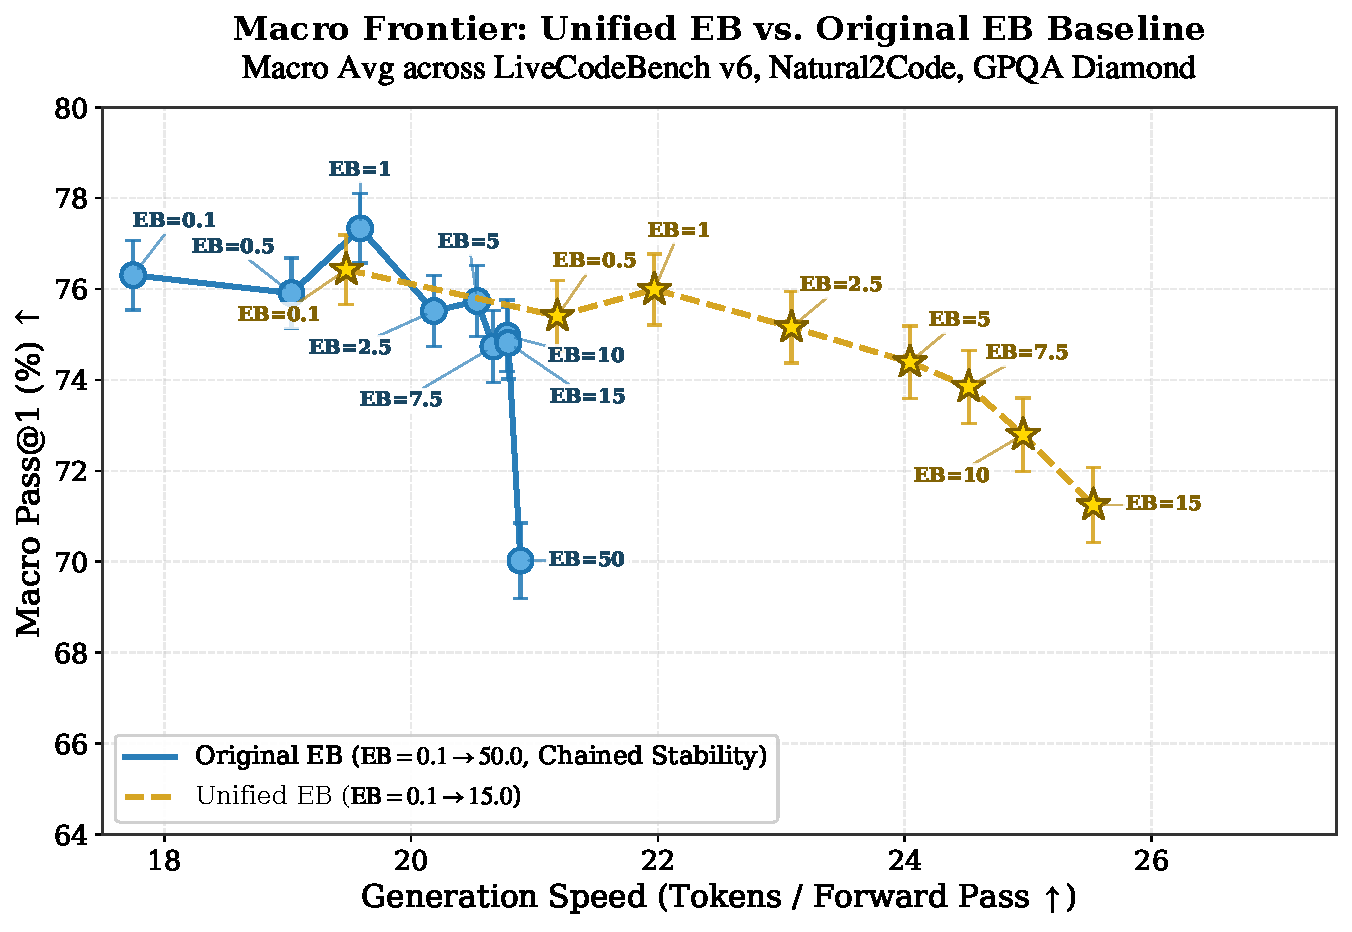
\includegraphics[height=\frontierheight]{images/fig_macro_frontier_original_vs_unified.pdf}
        \caption{Original vs.\ unified stopping.}
        \label{fig:unified-vs-orig}
    \end{subfigure}
    \hfill
    \begin{subfigure}[b]{0.51\textwidth}
        \centering
        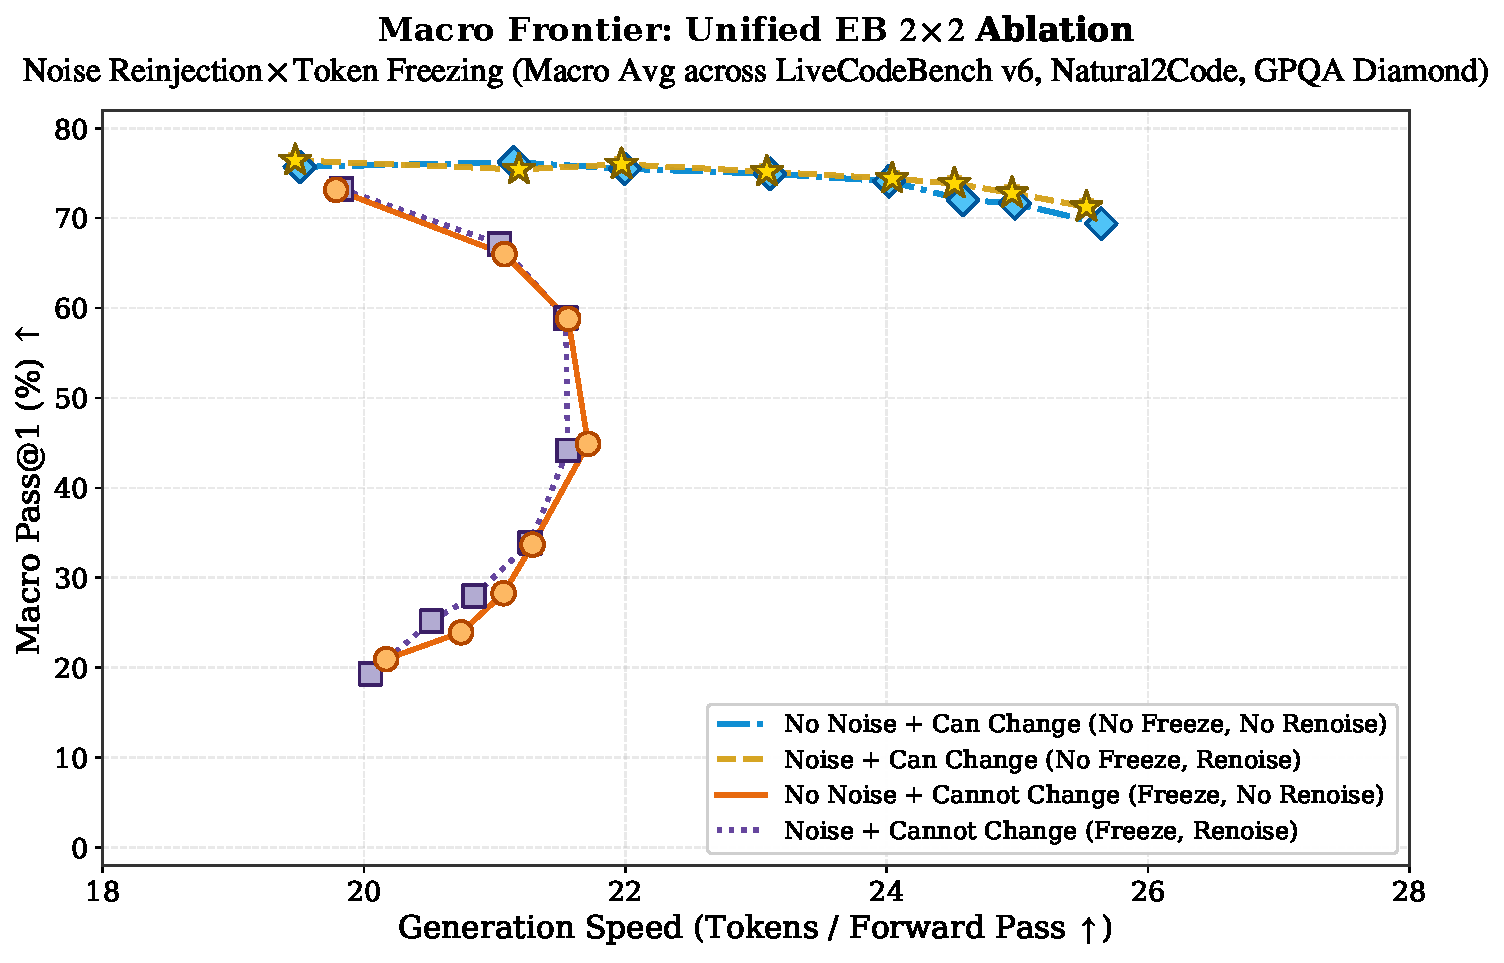
\includegraphics[height=\frontierheight]{images/fig_macro_frontier_unified_ablation_2x2.pdf}
        \caption{Frozen vs.\ base EB sampler.}
        \label{fig:frozen-eb-frontier}
    \end{subfigure}
    \caption{\textbf{(a)} The unified stopping criterion matches the original at a slight speedup. \textbf{(b)} Simulation of per-position commitment in DiffusionGemma: freezing each token upon acceptance removes the chance for later revision. Frozen variants degrade much faster than unfrozen variants as the entropy bound is relaxed, showing the cost of losing this sampler flexibility.}
    \label{fig:eb-frontiers}
\end{figure}

